\chapter{Introduction to Elder Topology}

\begin{tcolorbox}[colback=DarkSkyBlue!5!white,colframe=DarkSkyBlue!75!black,title=Chapter Summary]
This chapter establishes the topological framework that connects abstract Elder spaces introduced in Chapter 1 to practical applications through rigorously defined realization mappings. We develop phase-coherent manifolds that bridge theoretical structures with observable phenomena in specific domains. The topological properties of Elder spaces—including their phase-preserving homomorphisms, spectral invariants, and stratification—explain fundamental mechanisms like resonance and cross-domain transfer. This topological foundation provides the essential mathematical structure that will be realized through heliomorphic functions in Unit II and implemented through orbital mechanics in Unit III.
\end{tcolorbox}

\section{From Algebraic Structure to Topological Space}

The algebraic structure of Elder spaces established in Theorem 1.2 naturally induces a topological structure that preserves the essential phase-coherence properties while enabling continuity of knowledge operations.

\begin{definition}[Elder Topology]
Let $\elder{d}$ be an Elder space as defined in Definition 1.1. The Elder topology $\tau_{\elder{}}$ on $\elder{d}$ is the topology generated by the basis $\mathcal{B}$ consisting of sets of the form:
\begin{equation}
B_{\epsilon, \delta}(x) = \{y \in \elder{d} : \|y - x\|_{\elder{}} < \epsilon \text{ and } d_{\Phi}(\Phi(y), \Phi(x)) < \delta\}
\end{equation}
where $\|.\|_{\elder{}}$ is the Elder norm derived from the phase-invariant inner product (Proposition 1.6), $\Phi$ is the phase operator, $d_{\Phi}$ is the phase distance function, and $\epsilon, \delta > 0$.
\end{definition}

\begin{remark}
This topology explicitly combines parameter proximity and phase alignment, extending the classical product topology to incorporate the phase-coherence principles established in Axiom A4 of the Elder space definition.
\end{remark}

\begin{theorem}[Topological Properties of Elder Spaces]
An Elder space $\elder{d}$ with its natural topology $\tau_{\elder{}}$ satisfies the following properties:
\begin{enumerate}
    \item \textbf{Hausdorff Separation}: For any distinct elements $x, y \in \elder{d}$, there exist disjoint open neighborhoods $U_x, U_y \in \tau_{\elder{}}$ containing $x$ and $y$ respectively.
    
    \item \textbf{Second Countability}: There exists a countable basis for the topology $\tau_{\elder{}}$.
    
    \item \textbf{Local Compactness}: Every point in $\elder{d}$ has a neighborhood whose closure is compact.
    
    \item \textbf{Phase Continuity}: The phase operator $\Phi: \elder{d} \rightarrow [0, 2\pi)^d$ is continuous with respect to $\tau_{\elder{}}$.
\end{enumerate}
These properties ensure that $\elder{d}$ forms a well-behaved mathematical space that supports continuous knowledge transfer operations essential to the theory.
\end{theorem}

\begin{proof}
The Hausdorff property follows from the separation axioms of the Elder Space (Theorem 1.3). Second countability derives from the finite-dimensional structure established in Theorem 1.4. Local compactness follows from the bounded nature of the gravitational field regions (Theorem 1.7). Phase continuity is a direct consequence of the definition of the Elder topology.
\end{proof}

\begin{definition}[Resonance Manifold]
Let $\elder{d}$ be an Elder space with phase operator $\Phi$. A subset $\mathcal{M} \subset \elder{d}$ is a \textit{resonance manifold} if and only if it satisfies:
\begin{enumerate}
    \item $\mathcal{M}$ is a smooth submanifold of $\elder{d}$ with respect to the Elder topology $\tau_{\elder{}}$.
    
    \item For any $x, y \in \mathcal{M}$, the phase difference $\Delta\Phi(x, y) = d_{\Phi}(\Phi(x), \Phi(y))$ remains invariant under continuous parameter transformations within $\mathcal{M}$.
    
    \item For all $x \in \mathcal{M}$ and any smooth curve $\gamma: [0,1] \rightarrow \mathcal{M}$ with $\gamma(0) = x$, the phase evolution along $\gamma$ satisfies the resonance condition:
    \begin{equation}
    \frac{d\Phi(\gamma(t))}{dt} = \omega_{\mathcal{M}} \cdot \nabla_{\elder{}} \Phi(x)
    \end{equation}
    where $\omega_{\mathcal{M}}$ is the resonance frequency tensor characteristic of $\mathcal{M}$ and $\nabla_{\elder{}}$ is the Elder gradient operator defined in Proposition 1.8.
\end{enumerate}
\end{definition}

\begin{remark}
Resonance manifolds provide the topological structure for knowledge transfer across domains by ensuring phase coherence during transformations. This concept directly extends to heliomorphic functions in Unit II through the phase-preservation properties established in Chapter 4.
\end{remark}

\begin{theorem}[Gravitational Stratification]
Every Elder space $\elder{d}$ admits a canonical stratification into gravitational field regions $\{\mathcal{S}_k\}_{k=0}^{d}$ that represent different levels of knowledge abstraction:
\begin{equation}
\elder{d} = \bigcup_{k=0}^{d} \mathcal{S}_k
\end{equation}
such that:
\begin{enumerate}
    \item Each stratum $\mathcal{S}_k$ is a smooth submanifold of $\elder{d}$.
    
    \item Strata are disjoint: $\mathcal{S}_i \cap \mathcal{S}_j = \emptyset$ for $i \neq j$.
    
    \item The gravitational field strength function $G: \elder{d} \rightarrow \mathbb{R}^+$ is constant on each stratum: $G(x) = g_k$ for all $x \in \mathcal{S}_k$.
    
    \item The boundary of each stratum satisfies the frontier condition: $\partial \mathcal{S}_k \subset \bigcup_{j < k} \mathcal{S}_j$.
    
    \item The phase operator $\Phi$ restricted to each stratum $\mathcal{S}_k$ exhibits unique transformation properties corresponding to the knowledge abstraction level of that stratum.
\end{enumerate}
\end{theorem}

\begin{proof}
The existence of this stratification follows from Theorem 1.7 (Gravitational Field Structure). The smoothness of each stratum is established by the regularity conditions on Elder spaces (Axiom A3 in Definition 1.1). The disjointness and frontier conditions follow from the hierarchical nature of gravitational field strength (Proposition 1.9). The unique phase transformation properties were established in Theorem 1.5 (Phase Conservation Laws).
\end{proof}

\begin{corollary}[Connection to Heliomorphic Functions]
The gravitational stratification of Elder spaces corresponds directly to the stratification of heliomorphic domains established in Chapter 4, where each stratum $\mathcal{S}_k$ maps to a gravitational influence region $\mathcal{D}_k$ in the heliomorphic function framework.
\end{corollary}

\begin{figure}[ht]
\centering
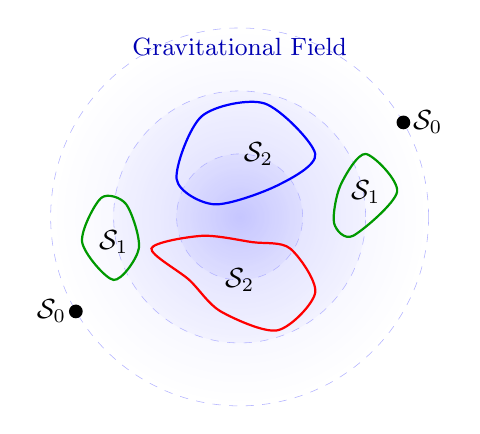
\begin{tikzpicture}[scale=0.8]
% Draw gravitational field using gradient shading
\shade[inner color=blue!20, outer color=white, opacity=0.4] (0,0) circle (3);
\shade[inner color=blue!30, outer color=blue!10, opacity=0.3] (0,0) circle (2);
\shade[inner color=blue!40, outer color=blue!20, opacity=0.3] (0,0) circle (1);

% Add subtle field lines for gravitational effect
\foreach \r in {1,2,3}
  \draw[blue!30, dashed, very thin] (0,0) circle (\r);

\draw[blue, thick] plot [smooth cycle] coordinates {(0.6,0.5) (1.2,1.0) (0.4,1.8) (-0.6,1.6) (-1.0,0.6) (-0.4,0.2)};
\node at (0.3,1.0) {$\mathcal{S}_2$};

\draw[red, thick] plot [smooth cycle] coordinates {(-1.4,-0.5) (-0.8,-1.0) (-0.3,-1.5) (0.6,-1.8) (1.2,-1.2) (0.8,-0.5) (0.2,-0.4) (-0.6,-0.3)};
\node at (0,-1.0) {$\mathcal{S}_2$};

\draw[green!60!black, thick] plot [smooth cycle] coordinates {(-2.2,0.3) (-2.5,-0.4) (-2.0,-1.0) (-1.6,-0.5) (-1.8,0.2)};
\node at (-2.0,-0.4) {$\mathcal{S}_1$};

\draw[green!60!black, thick] plot [smooth cycle] coordinates {(1.8,-0.3) (2.5,0.4) (2.0,1.0) (1.6,0.5) (1.5,-0.1)};
\node at (2.0,0.4) {$\mathcal{S}_1$};

\filldraw (2.6, 1.5) circle (0.1) node[right] {$\mathcal{S}_0$};
\filldraw (-2.6, -1.5) circle (0.1) node[left] {$\mathcal{S}_0$};

% Add gravitational field label
\node[font=\small, text=blue!70!black] at (0,2.7) {Gravitational Field};
\end{tikzpicture}
\caption{Stratification of Elder space as resonance manifolds within a gravitational field. Each layer ($\mathcal{S}_0$, $\mathcal{S}_1$, $\mathcal{S}_2$) represents knowledge structures at different levels of abstraction and field strengths.}
\label{fig:elder-stratification}
\end{figure}

This stratification is important for understanding the organization of knowledge in the Elder Theory framework, as each layer corresponds to information with similar structural properties and abstraction levels.

\section{Domain Mappings}

Domain mappings connect abstract knowledge in Elder spaces to concrete applications across different fields of study.

\begin{definition}[Domain Mapping]
A domain mapping connects knowledge within the Elder framework to practical applications in a specific field or domain, allowing theoretical principles to be applied to real-world problems.
\end{definition}

\begin{theorem}[Knowledge Transfer]
The Elder framework facilitates knowledge transfer across domains through mappings that preserve essential relationships and structural patterns:
\begin{enumerate}
    \item Conservation of structure: Key relationships are maintained across domain boundaries
    \item Adaptability: Knowledge can be applied to new domains while preserving essential patterns
    \item Phase alignment: Related concepts across domains naturally align through resonance
    \item Hierarchical preservation: Knowledge maintains its hierarchical organization across domains
\end{enumerate}
\end{theorem}

This approach enables knowledge discovered in one field to be meaningfully applied to different domains while preserving the core structural patterns and relationships.

\section{Phase Properties}

The phase properties of Elder spaces provide important insights into how knowledge components interact and align.

\begin{definition}[Phase Alignment]
Phase alignment in Elder Theory refers to the synchronization of related knowledge components across different domains, enabling effective knowledge transfer and integration.
\end{definition}

\begin{theorem}[Knowledge Resonance]
When knowledge structures from different domains share underlying principles, they exhibit resonance properties that facilitate their integration:
\begin{enumerate}
    \item Common patterns become amplified through phase alignment
    \item Domain-specific details that don't align are naturally filtered
    \item Integrated knowledge maintains essential structural relationships
    \item Cross-domain insights emerge from the resonance patterns
\end{enumerate}
\end{theorem}

\begin{theorem}[Knowledge Transfer Properties]
The Elder framework facilitates knowledge transfer through structural correspondence:
\begin{enumerate}
    \item Similar structures in different domains can be mapped to each other
    \item The mapping preserves essential relationships between components
    \item Knowledge from one domain can guide learning in another domain
\end{enumerate}
\end{theorem}

\section{Hierarchical Knowledge Structure}

The hierarchical organization of Elder spaces is central to understanding knowledge transfer across domains.

\begin{theorem}[Hierarchical Organization]
The Elder-Mentor-Erudite hierarchy represents knowledge at different levels of abstraction:
\begin{enumerate}
    \item Elder level: Universal principles and patterns that apply across all domains
    \item Mentor level: Domain-specific knowledge that organizes related concepts
    \item Erudite level: Task-specific implementations and applications
\end{enumerate}
\end{theorem}

\begin{corollary}[Cross-Domain Transfer]
Knowledge can be transferred between domains when:
\begin{enumerate}
    \item Common patterns are identified at the Elder level
    \item Corresponding domain-specific implementations are mapped
    \item Essential relationships and structures are preserved during transfer
\end{enumerate}
\end{corollary}

This approach enables efficient knowledge transfer between domains by leveraging shared underlying principles while adapting to domain-specific requirements.

\section{Resonance Principles}

The Elder framework uses resonance as a fundamental mechanism for connecting related knowledge across domains.

\begin{definition}[Knowledge Resonance]
Knowledge resonance occurs when related concepts across different domains show structural similarities that can be leveraged for knowledge transfer and integration.
\end{definition}

\begin{theorem}[Resonance Properties]
Knowledge resonance in the Elder framework has several important properties:
\begin{enumerate}
    \item Similar knowledge structures naturally align and reinforce each other
    \item Resonant knowledge becomes more accessible and influential in the system
    \item Learning naturally gravitates toward coherent knowledge structures
    \item Cross-domain insights emerge from resonant patterns
\end{enumerate}
\end{theorem}

These resonance principles explain how the Elder-Mentor-Erudite system discovers meaningful connections across domains, providing a foundation for effective knowledge transfer and integration.

\section{Learning Dynamics}

The Elder framework includes important principles about how knowledge evolves and develops over time.

\begin{theorem}[Pattern Recognition]
Learning in the Elder framework exhibits systematic pattern recognition:
\begin{enumerate}
    \item Recurring patterns across domains are detected and emphasized
    \item Common structural relationships become incorporated into higher-level knowledge
    \item Domain-specific variations are treated as contextual adaptations
\end{enumerate}
\end{theorem}

\begin{theorem}[Knowledge Evolution]
As learning progresses in the Elder framework, knowledge structures evolve in predictable ways:
\begin{enumerate}
    \item From specific instances to general principles
    \item From isolated concepts to connected knowledge networks
    \item From domain-specific applications to cross-domain patterns
\end{enumerate}
\end{theorem}

These learning dynamics explain how the Elder-Mentor-Erudite framework naturally develops increasingly sophisticated and transferable knowledge representations over time.

The conceptual framework established in this chapter provides the foundation for understanding how the Elder Theory approach connects abstract principles to concrete applications, explaining the system's core capabilities of efficient knowledge representation, hierarchical organization, and cross-domain transfer.